\PassOptionsToPackage{hidelinks}{hyperref}

\documentclass[stu,12pt,floatsintext]{apa7} % man doc stu jou

\usepackage[american]{babel}

\usepackage{csquotes} 
\usepackage[style=apa,sortcites=true,sorting=nyt,backend=biber]{biblatex}

\DeclareLanguageMapping{american}{american-apa}
% \addbibresource{bibliography.bib} 
\usepackage[T1]{fontenc} 
\usepackage{ctex}
\usepackage{xeCJK}
\usepackage{mathptmx} % This is the Times New Roman font, which was the norm back in my day. If you'd like to use a different font, the options are laid out here: https://www.overleaf.com/learn/latex/Font_typefaces
% Alternately, you can comment out or delete these two commands and just use the Overleaf default font. So many choices!
\setCJKmainfont{Songti SC Regular} % 设置中文主字体为 STSong,字间距增加
\setmainfont{Times New Roman} % 设置英文字体
% \renewcommand{\today}{\number\year 年 \number\month 月 \number\day 日}

%公式和列表
\usepackage{enumitem}
\usepackage{amsmath}
\usepackage{amsthm} 
\usepackage{amssymb}
\addtolength{\jot}{5pt}

%绘图用
\usepackage{caption}   % 图片脚注
\usepackage{graphicx}  
\usepackage{caption}
\usepackage{subfigure} % 子图包


\usepackage{pythonhighlight}

% Set up fancy header/footer
\usepackage{fancyhdr}
\pagestyle{fancy}
\fancyhead[LO,L]{2025年春学期}
\fancyhead[CO,C]{贝叶斯统计学基础}
\fancyhead[RO,R]{\number\year 年 \number\month 月 \number\day 日}
\fancyfoot[LO,L]{}
\fancyfoot[CO,C]{\thepage}
\fancyfoot[RO,R]{}
\renewcommand{\headrulewidth}{0.4pt}
\renewcommand{\footrulewidth}{0.4pt}


% Title page stuff _____________________
\title{APA Format Starter Paper, Tailored to Lab Reports But Adaptable to Other Writing Assignments} % The big, long version of the title for the title page
\shorttitle{APA Starter} % The short title for the header
\author{Your Name Here}
\duedate{April 20, 2024}
% \date{January 17, 2024} The student version doesn't use the \date command, for whatever reason
\affiliation{Your School}
\course{PSY 4321} % LaTeX gets annoyed (i.e., throws a grumble-error) if this is blank, so I put something here. However, if your instructor will mark you off for this being on the title page, you can leave this entry blank (delete the PSY 4321, but leave the command), and just make peace with the error that will happen. It won't break the document.
\professor{Dr. Professor}  % Same situation as for the course info. Some instructors want this, some absolutely don't and will take off points. So do what you gotta.

\abstract{This is the abstract for this paper, wherein the main points of the introduction, method, results, and discussion are quickly talked about. Probably in more than one sentence, though. Dare I guess, more than two? There is a page break before starting the Introduction.}

%\keywords{APA style, demonstration} % If you need to have keywords for your paper, delete the % at the start of this line


\begin{document}
\begin{titlepage}
    \centering
    \vspace*{4cm} % 调整标题的垂直位置
    \Huge
    {\heiti 贝叶斯统计学基础作业2} \\
    \vspace{1cm}
    \Large
    毛沛炫\ \ \ 3220102692 \\
    \vspace{12.3cm}
    \Large
    % \today
    \number\year 年 \number\month 月 \number\day 日
    \vfill
\end{titlepage}

\xeCJKsetup{CJKglue={\hskip 0.8pt plus 0.08\baselineskip}}

\noindent 1. {\heiti 假定对于二项分布参数\textit{p}我们采用均匀先验分布,并且在 10次试验中观察到了 4 次正性结果,}
\begin{enumerate}[itemsep=2pt,topsep=0pt,parsep=0pt,label=(\alph*)]
\item  给出先验贝塔分布的参数值(2 分)

\item  给出后验贝塔分布的参数值(2 分)
    
\item  给出在先验分布下二项分布参数 \textit{p} 的期望值(2 分)
    
\item  给出样本中正性结果的比例(2 分)
    
\item  给出二项分布参数 \textit{p} 的极大似然估计值(2 分)
    
\item  给出在后验分布下二项参数 \textit{p} 的期望值,并以先验分布下该参数的期望值和该参数的极大似然估计值的加权平均形式表达(4 分)
\end{enumerate}


\noindent \textbf{解答:}
\begin{enumerate}[itemsep=2pt,topsep=0pt,parsep=0pt,label=(\alph*)]
    \item 先验贝塔分布的参数值
    
    \(\alpha = 1\) 和 \(\beta = 1\)。见图\ref{fig:beta11}
    \vspace{-0.4cm}
    \begin{figure}
        \centering
        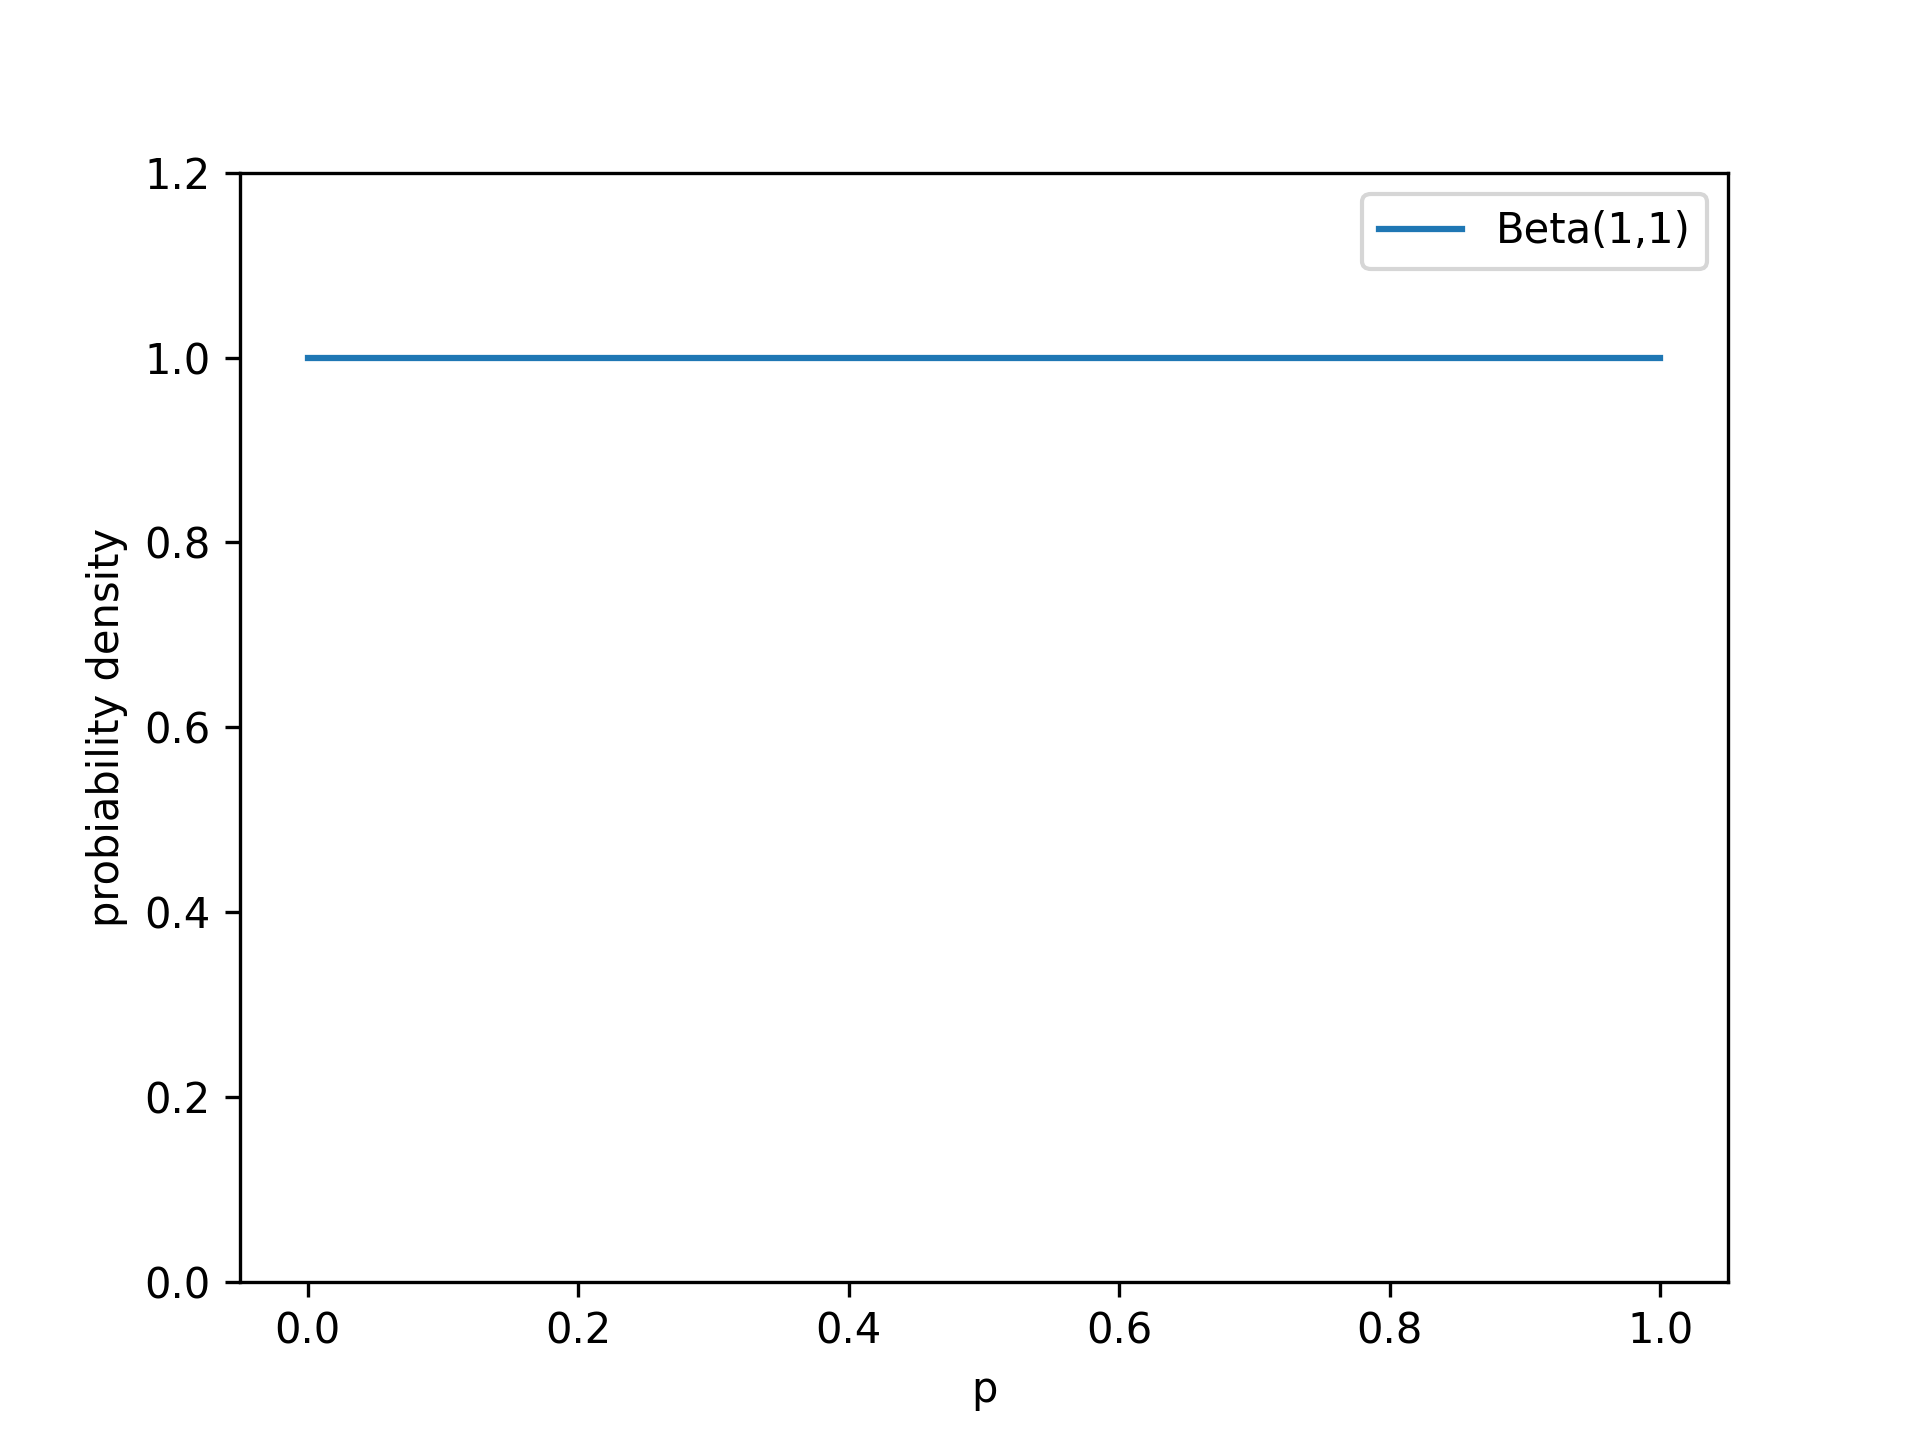
\includegraphics[width=0.6\linewidth]{figure/beta11.png} % Replace with the actual path to your image
        \caption{先验贝塔分布的参数值} % Replace with your caption
        \label{fig:beta11} % Ensure the label is inside the figure environment
        \vspace{-2em}
    \end{figure}

    \item 后验贝塔分布的参数值
    

    \begin{figure}
        \vspace{-1em}
        \centering
        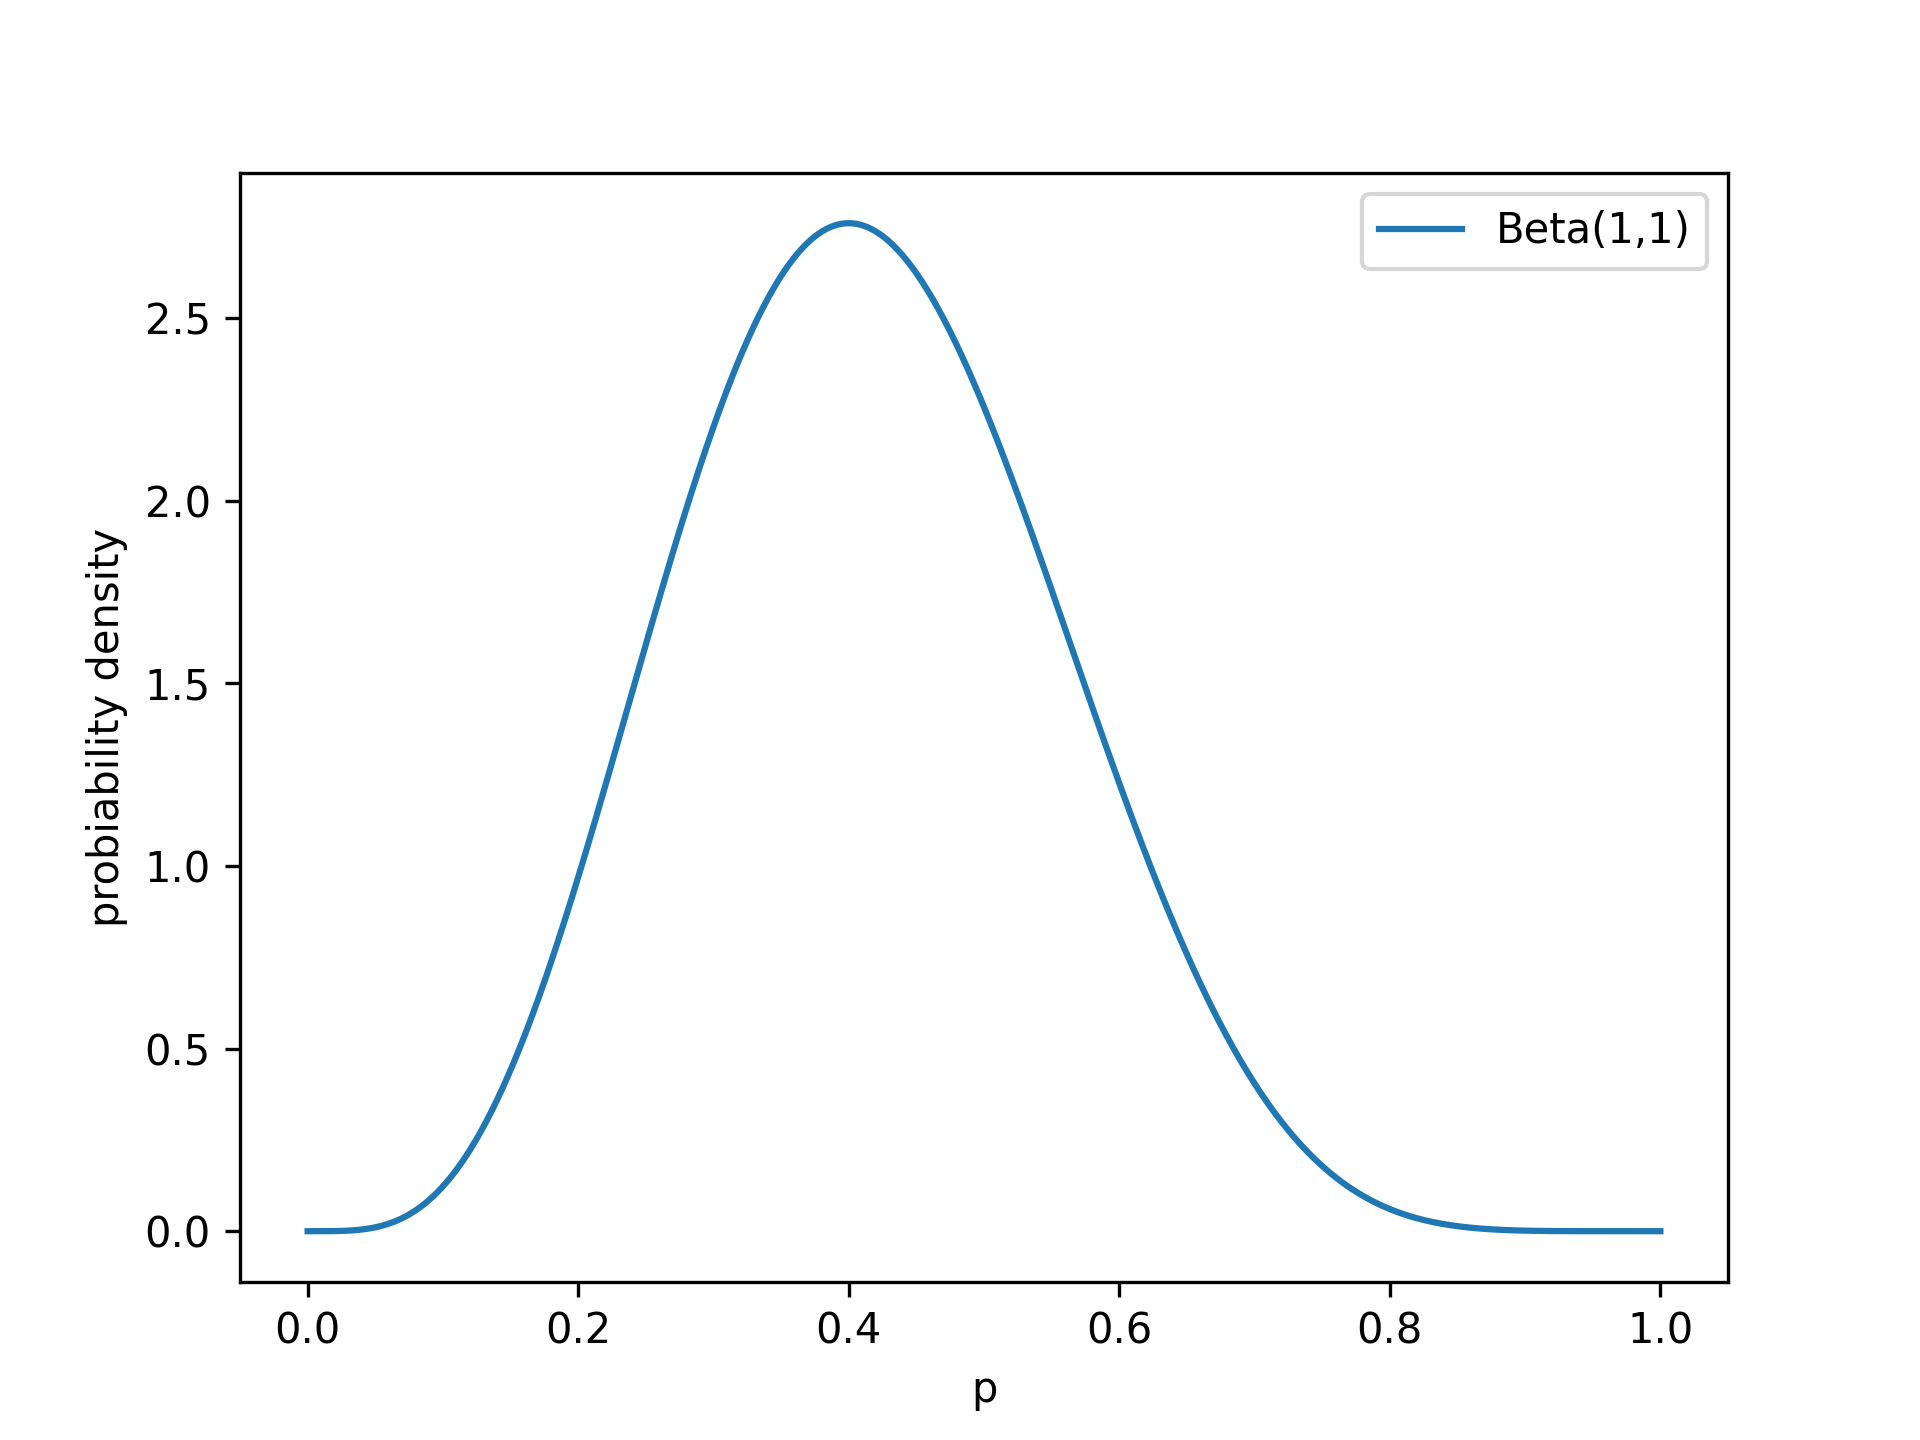
\includegraphics[width=0.6\linewidth]{figure/beta57.png} 
        \caption{后验贝塔分布的参数值}
        \label{fig:beta57}
        \vspace{-2em}
    \end{figure}

    后验贝塔分布的参数为 \(\alpha = 5\) 和 \(\beta = 7\)。
    \setlength\abovedisplayskip{0.7em}
    \setlength\belowdisplayskip{0.7em}
    \[
    \alpha_{\text{后验}} = \alpha + \text{正性结果数} = 1 + 4 = 5
    \]
    \[
    \beta_{\text{后验}} = \beta + \text{负性结果数} = 1 + 6 = 7
    \]


    \item 给出先验分布下二项分布参数 \textit{p} 的期望值
    
    先验分布为均匀分布,其期望值为:
    \setlength\abovedisplayskip{0.7em}
    \setlength\belowdisplayskip{0.7em}
    \[
    \text{E}[p] = \frac{\alpha}{\alpha + \beta} = \frac{1}{1 + 1} = 0.5
    \]

    \item 给出样本中正性结果的比例
    
    样本中正性结果的比例为\(4 / 10 = 0.4\)
    
    \item  给出二项分布参数 \textit{p} 的极大似然估计值
    

    在 10 次试验中观察到 4 次正性结果,其似然函数为:
    \setlength\abovedisplayskip{0.7em}
    \setlength\belowdisplayskip{0.7em}
    \[
    L(p) = P(X = 4) = \binom{10}{4} p^4 (1-p)^{6}
    \]

    为了求极大似然估计值,我们对似然函数取对数,得到对数似然函数:
    \[
    \setlength\abovedisplayskip{0.7em}
    \setlength\belowdisplayskip{0.7em}
    \ln L(p) = \ln \binom{10}{4} + 4 \ln p + 6 \ln (1-p)
    \]

    对 \(p\) 求导并令导数为零:
    \[
    \setlength\abovedisplayskip{0.7em}
    \setlength\belowdisplayskip{0.7em}
    \frac{d}{dp} \ln L(p) = \frac{4}{p} - \frac{6}{1-p} = 0
    \]

    解得:
    \[
    \setlength\abovedisplayskip{0.7em}
    \setlength\belowdisplayskip{0.7em}
    p = \frac{4}{10} = 0.4
    \]

    因此,二项分布参数 \(p\) 的极大似然估计值为:
    \setlength\abovedisplayskip{0.7em}
    \setlength\belowdisplayskip{0.7em}
    \[
    \hat{p}_{\text{MLE}} = 0.4
    \]
    
    \item  给出在后验分布下二项参数 \textit{p} 的期望值,并以先验分布下该参数的期望值和该参数的极大似然估计值的加权平均形式表达
    \[
    \text{E}[p \mid D] = \frac{\alpha_{\text{后验}}}{\alpha_{\text{后验}} + \beta_{\text{后验}}} = \frac{5}{5 + 7} = \frac{5}{12} 
    \]
    
    这个期望值可以表示为:
    \setlength\abovedisplayskip{0.7em}
    \setlength\belowdisplayskip{0.7em}
    \[
    \text{E}[p \mid D] = \frac{\alpha + \text{正性结果数}}{\alpha + \beta + \text{总试验数}} = \frac{1 + 4}{1 + 1 + 10} = \frac{5}{12}
    \]
    
    也可以表示为先验期望值和极大似然估计值的加权平均:
    \setlength{\abovedisplayskip}{0.5em}
    \setlength{\belowdisplayskip}{0.5em}
    \[
        \text{E}[p \mid D] = \frac{2 \times 0.5 + 10 \times 0.4}{2 + 10} = \frac{1 + 4}{12} = \frac{5}{12} 
    \]
    其中,先验权重为 \(\alpha + \beta = 2\),数据权重为试验次数 \(n = 10\)。
\end{enumerate}

\noindent 2. {\heiti 假定对于二项分布参数\(p\),我们有三个假设:
\setlength\abovedisplayskip{0.7em}
\setlength\belowdisplayskip{0.7em}
\[H_0:p = 0.5, \ \ H_1:p=0.4,\ \ H_2:p \thicksim unif(0,1)\]
\ \ \ \  另外,我们进行了 50 次伯努利试验,得到了 20 次正性结果,}

\begin{enumerate}[itemsep=2pt,topsep=0pt,parsep=0pt,label=(\alph*)]
    \item 求对于每个假设的\(P(D \mid H)\)(6 分)
    \item 求各对假设间的贝叶斯因子(3 分)
    \item 根据以上结果,我们能够做出怎样的统计推断(2 分)
    \item 为了能够做出接受上述三个假设中某一假设的统计推断,在假定样本正性结果比例不变的情况下,还需进行多少次额外的伯努利试验(5 分)
\end{enumerate}

\noindent \textbf{解答:}

\hspace{2.2em}以\(\sqrt{10}\)为标准

\begin{enumerate}[itemsep=2pt,topsep=0pt,parsep=0pt,label=(\alph*)]

    \item 求对于每个假设的\(P(D \mid H)\)
    
    记\(n = 50,\ \ z = 20\),对\(H_0\)和\(H_1\),我们有:
    \setlength\abovedisplayskip{0.7em}
    \setlength\belowdisplayskip{0.7em}  
    \[
    P(D \mid H) =  p^z (1-p)^{n-z} 
    \]
    对于\(H_0\),\(p = 0.5\),\(P(D \mid H_0) = 0.5^{20} \times 0.5^{30} = 0.5^{50} \approx 8.88\text{E}-16\),

    对于\(H_1\),\(p = 0.4\),\(P(D \mid H_1) = 0.4^{20} \times 0.6^{30}\approx 2.43\text{E}-15\),

    对于\(H_2\),
    \setlength\abovedisplayskip{0.7em}
    \setlength\belowdisplayskip{0.7em}
    \begin{align*}
        P(D \mid H_2) & = \int_{0}^{1} L(D|p)f(p)dp\\
         & = \int_0^1 p^{20} (1-p)^{30} dp = \frac{1}{2403589824441960}
    \end{align*}

    \item 求各对假设间的贝叶斯因子
    \setlength\abovedisplayskip{0.7em}
    \setlength\belowdisplayskip{0.7em}
    \begin{align*}
        BF_{01} & = \frac{0.5^{50}}{0.4^{20} \times 0.6^{30}} \approx 0.365\\
        BF_{02} & = \frac{0.5^{50}}{1/2403589824441960} \approx 2.135\\
        BF_{12} & = \frac{0.4^{20} \times 0.6^{30}}{1/2403589824441960} \approx 5.842
    \end{align*}

    \item 根据以上结果,我们能够做出怎样的统计推断
    
    由\(BF_{01}\),表明$H_0$和$H_1$之间,数据有较弱的证据支持 \(H_1\) 

    由\(BF_{02}\),表明$H_0$和$H_2$之间,数据有较弱的证据支持 \(H_0\)

    由\(BF_{12}\),表明$H_1$和$H_2$之间,数据有中等程度的证据支持 \(H_1\) 

    \item 为了能够做出接受上述三个假设中某一假设的统计推断,在假定样本正性结果比例不变的情况下,还需进行多少次额外的伯努利试验
    
    首先证明各贝叶斯因子的单调性。
    \begin{proof}\textbf{\(BF_{10}\)单调}
    
    \begin{align*}
        BF_{10(n+5)}-BF_{10(n)} & = \frac{0.4^{0.4n+2} \times 0.6^{0.6n+3}}{0.5^{n+5}} - \frac{0.4^{0.4n} \times 0.6^{0.6n}}{0.5^{n}}\\
        & = \frac{2^{n+5}\times 2^{0.4n+2}\times 3^{0.6n+3}}{5^{n+5}} - \frac{2^{n}\times 2^{0.4n}\times 3^{0.6n}}{5^{n}}\\
        & = \frac{\left(2^{n}\times 2^{0.4n}\times 3^{0.6n}\right)\left( 2^5\times 2^2 \times 3^3 - 5^5 \right)}{5^{n+5}}.
    \end{align*}

    \begin{align*}
    \because & \ 2^5\times 2^2 \times 3^3 - 5^5 = 3787 > 0 \\
    \therefore & \ BF_{10(n+5)}-BF_{10(n)} > 0\\
    \therefore & \ BF_{10} \text{单调递增}
    \end{align*}
        
    \end{proof}
    

    \begin{proof}
    \(BF_{12}\)单调
    \begin{align*}
        BF_{12(n+5)}-BF_{12(n)} & = \frac{0.4^{0.4n+2} \times 0.6^{0.6n+3}}{\int_0^1 p^{0.4n+2} (1-p)^{0.6n+3} dp} - \frac{0.4^{0.4n} \times 0.6^{0.6n}}{\int_0^1 p^{0.4n} (1-p)^{0.6n} dp}\\
    \end{align*}
    
    Sympy(代码见附录\ref{code1})给出\(\int_0^1 p^{0.4n} (1-p)^{0.6n} dp = \displaystyle \frac{\Gamma\left(0.4 n + 1\right) {{}_{2}F_{1}\left(\begin{matrix} - 0.6 n, 0.4 n + 1 \\ 0.4 n + 2 \end{matrix}\middle| {1} \right)}}{\Gamma\left(0.4 n + 2\right)}\)
    
    \vspace{0.2\baselineskip}
    因为我看不懂这个表达式,所以还是向python求助
    
    定义\(n\)为正整数且为5的倍数,计算\(BF_{12(n+5)}-BF_{12(n)}\),得到(代码见附录\ref{code2})
    \begin{align*}
        BF_{12(n+5)}-BF_{12(n)} & = \frac{{0.4}^{0.4 n + 2} {0.6}^{0.6 n + 3} \left( n + 6\right)!}{\left(0.4 n + 2\right)! \left(0.6 n + 3\right)!} - \frac{{0.4}^{0.4 n} {0.6}^{0.6 n} \left( n + 1\right)!}{\left(0.4 n\right)! \left(0.6 n\right)!}\\
        \frac{BF_{12(n+5)}-BF_{12(n)}}{{0.4}^{0.4 n} {0.6}^{0.6 n} \frac{\left( n + 1\right)!}{\left(0.4 n\right)! \left(0.6 n\right)!}} & =  \frac{{2}^{2} {3}^{3} (n+2)(n+3)(n+4)(n+5)(n+6)}{5^5(0.4 n + 1)(0.4 n + 2) (0.6 n + 1)(0.6 n + 2)(0.6 n + 3)} - 1\\
        & = \frac{(2n+4)(2n+6)(3n+12)(3n+18)}{(2n+5)(2n+10)(3n+5)(3n+10)}-1\triangleq f(n)
    \end{align*}


    使用sympy判断正负性(代码见附录\ref{code3}),输出\\
    f(n) > 0 when: True\\
    f(n) < 0 when: False

    因此,在n可能的取值中,
    \[\frac{(2n+4)(2n+6)(3n+12)(3n+18)}{(2n+5)(2n+10)(3n+5)(3n+10)}-1>0\]恒成立,所以\(BF_{12}\)单调递增
    \end{proof}

    \begin{proof}
    \(BF_{20}\)单调
    \begin{align*}
        BF_{20(n+5)}-BF_{20(n)} & = \frac{\int_0^1 p^{0.4n+2} (1-p)^{0.6n+3} dp}{0.5^{n+5}} - \frac{\int_0^1 p^{0.4n} (1-p)^{0.6n} dp}{0.5^{n}}\\
        & = \frac{{2}^{n + 5} \left(0.4 n + 2\right)! \left(0.6 n + 3\right)!}{\left( n + 6\right)!} - \frac{ {2}^{n} \left(0.4 n\right)! \left(0.6 n\right)!}{\left( n + 1\right)!}\\
        \frac{BF_{20(n+5)}-BF_{20(n)}}{\frac{2^5(0.4n)!(0.6n)!}{(n+1)!}} & =\frac{2^5(0.4n+1)(0.4n+2)(0.6n+1)(0.6n+2)(0.6n+3)}{(n+2)(n+3)(n+4)(n+5)(n+6)}-1\\
        & \triangleq f(n)
    \end{align*}

    使用sympy判断正负性,输出\\
    f(n) > 0 when: 20.936805530704 < n\\
    f(n) < 0 when: n < 20.936805530704

    因此,当\(n>50\)时,\(BF_{20}\)单调递增
    \end{proof}

    
    绘制贝叶斯因子随试验次数的变化曲线,如图\ref{fig:BF}所示。计算得出(代码见附录\ref{code4}),当试验次数达到 60 次时,贝叶斯因子 \(BF_{10}> 10^{1/2}\),即有中等程度的证据支持 \(H_2\)。\(BF_{10}\)在50-95次实验中的变化见图\ref{fig:BF10}。当总的实验次数\(n \geq 60\)时,不论是和\(H_0\)还是和\(H_2\)相比,数据都有数据有中等程度的证据支持\(H_1\)。\\
    
    \vspace{0.5\baselineskip}
    因此还需要进行10次额外的伯努利实验。

    \begin{figure}[htb]
        \centering
        \subfigure[贝叶斯因子随试验次数的变化曲线]{
            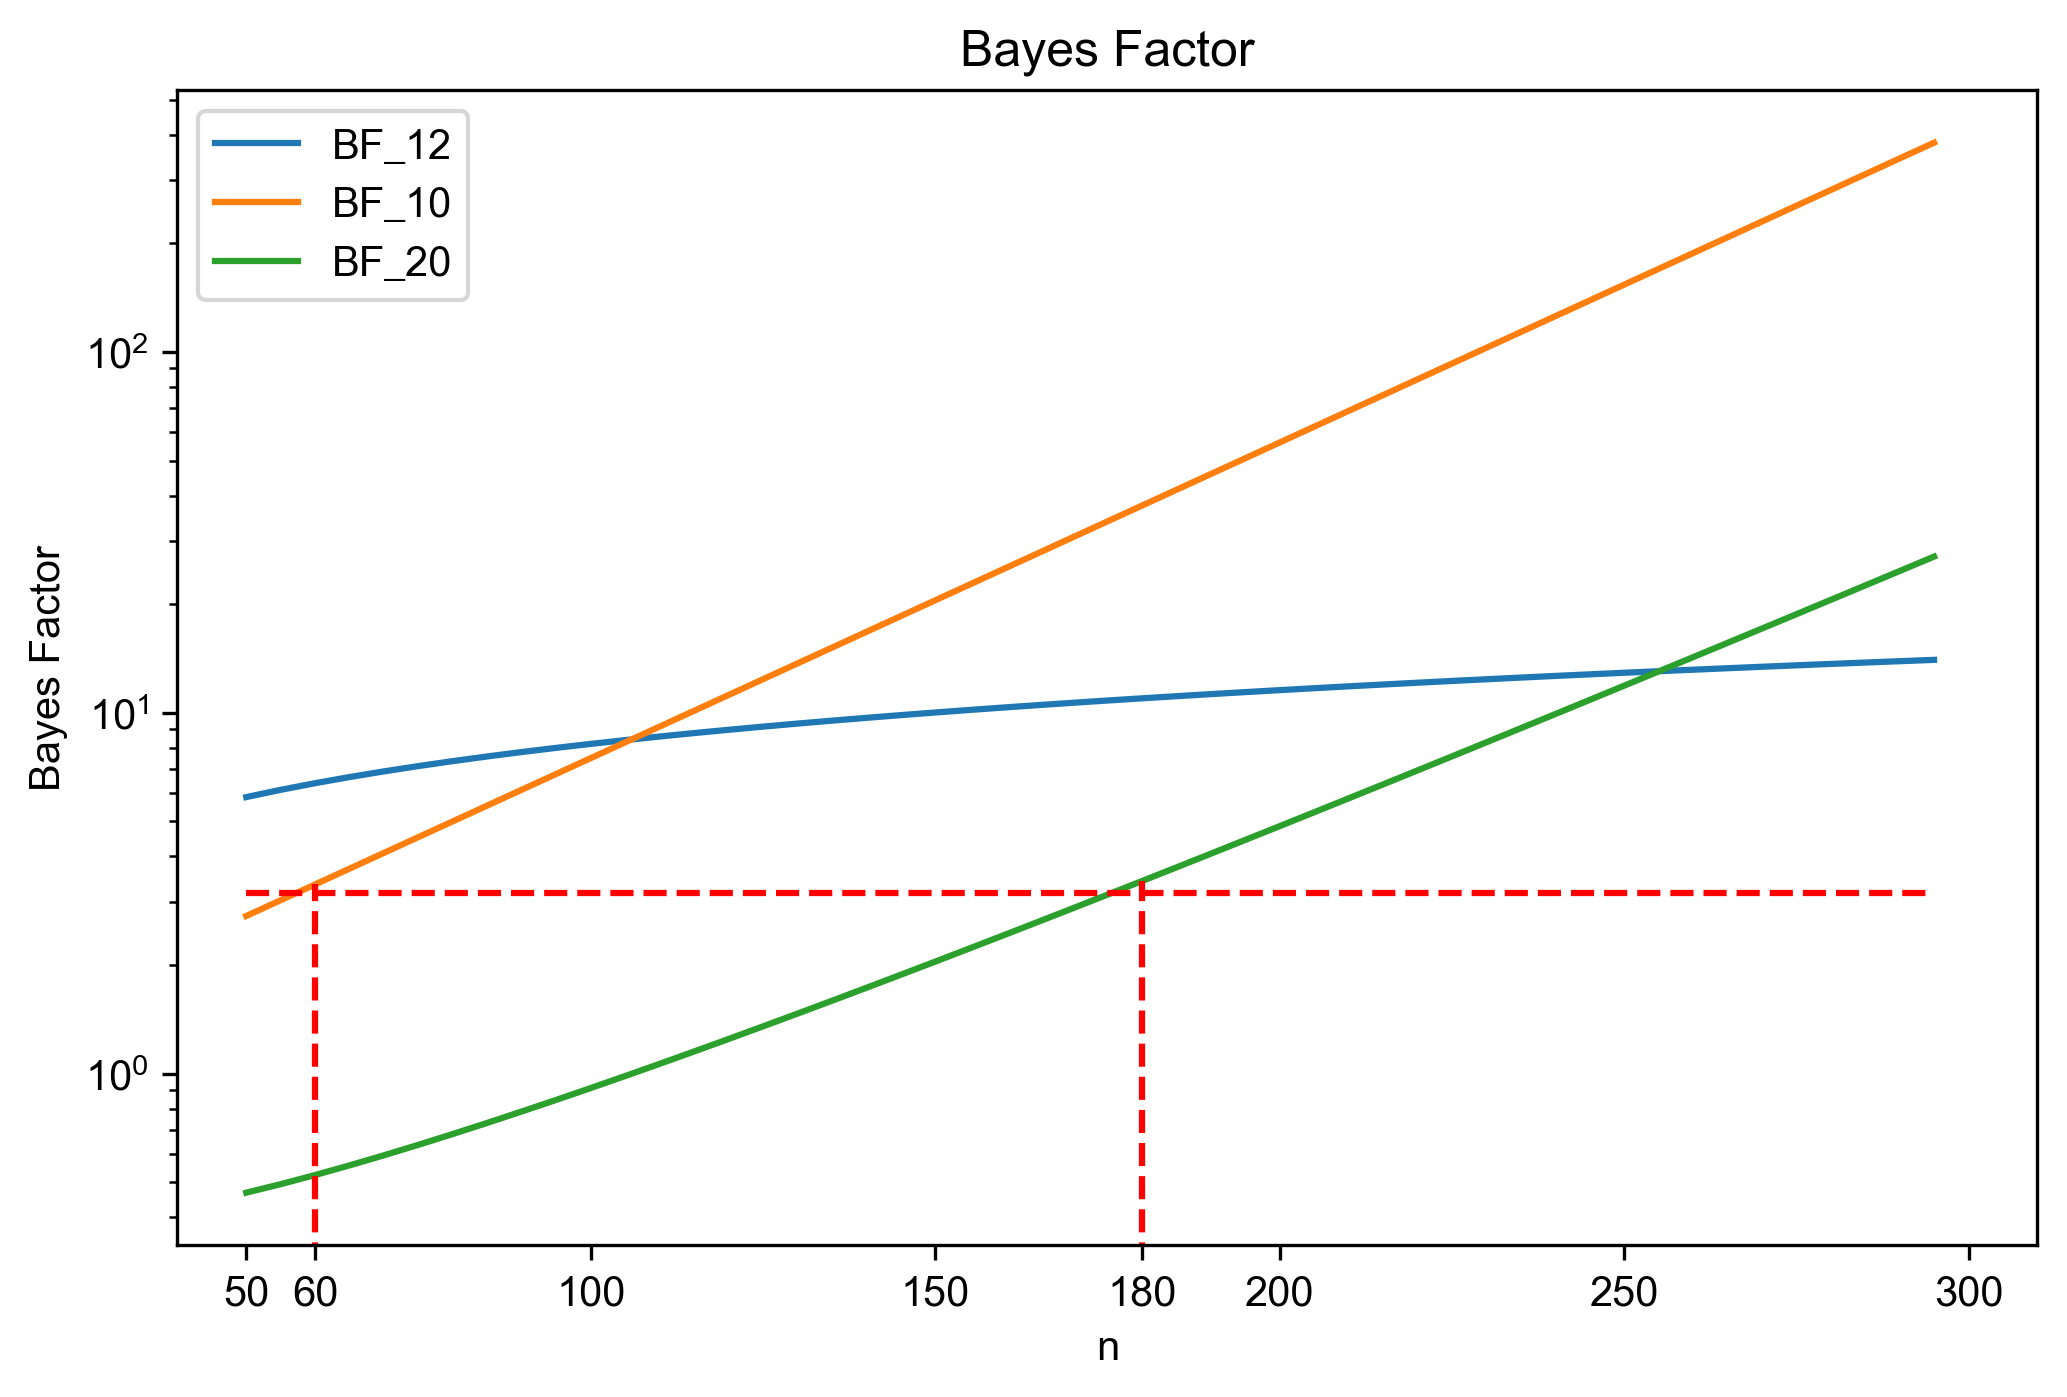
\includegraphics[width=0.7\linewidth]{figure/BF_0_400.png} % 替换为实际图片路径
            \label{fig:BF}
        }
        \hfill
        \subfigure[\(BF_{10}\)随试验次数的变化曲线]{
            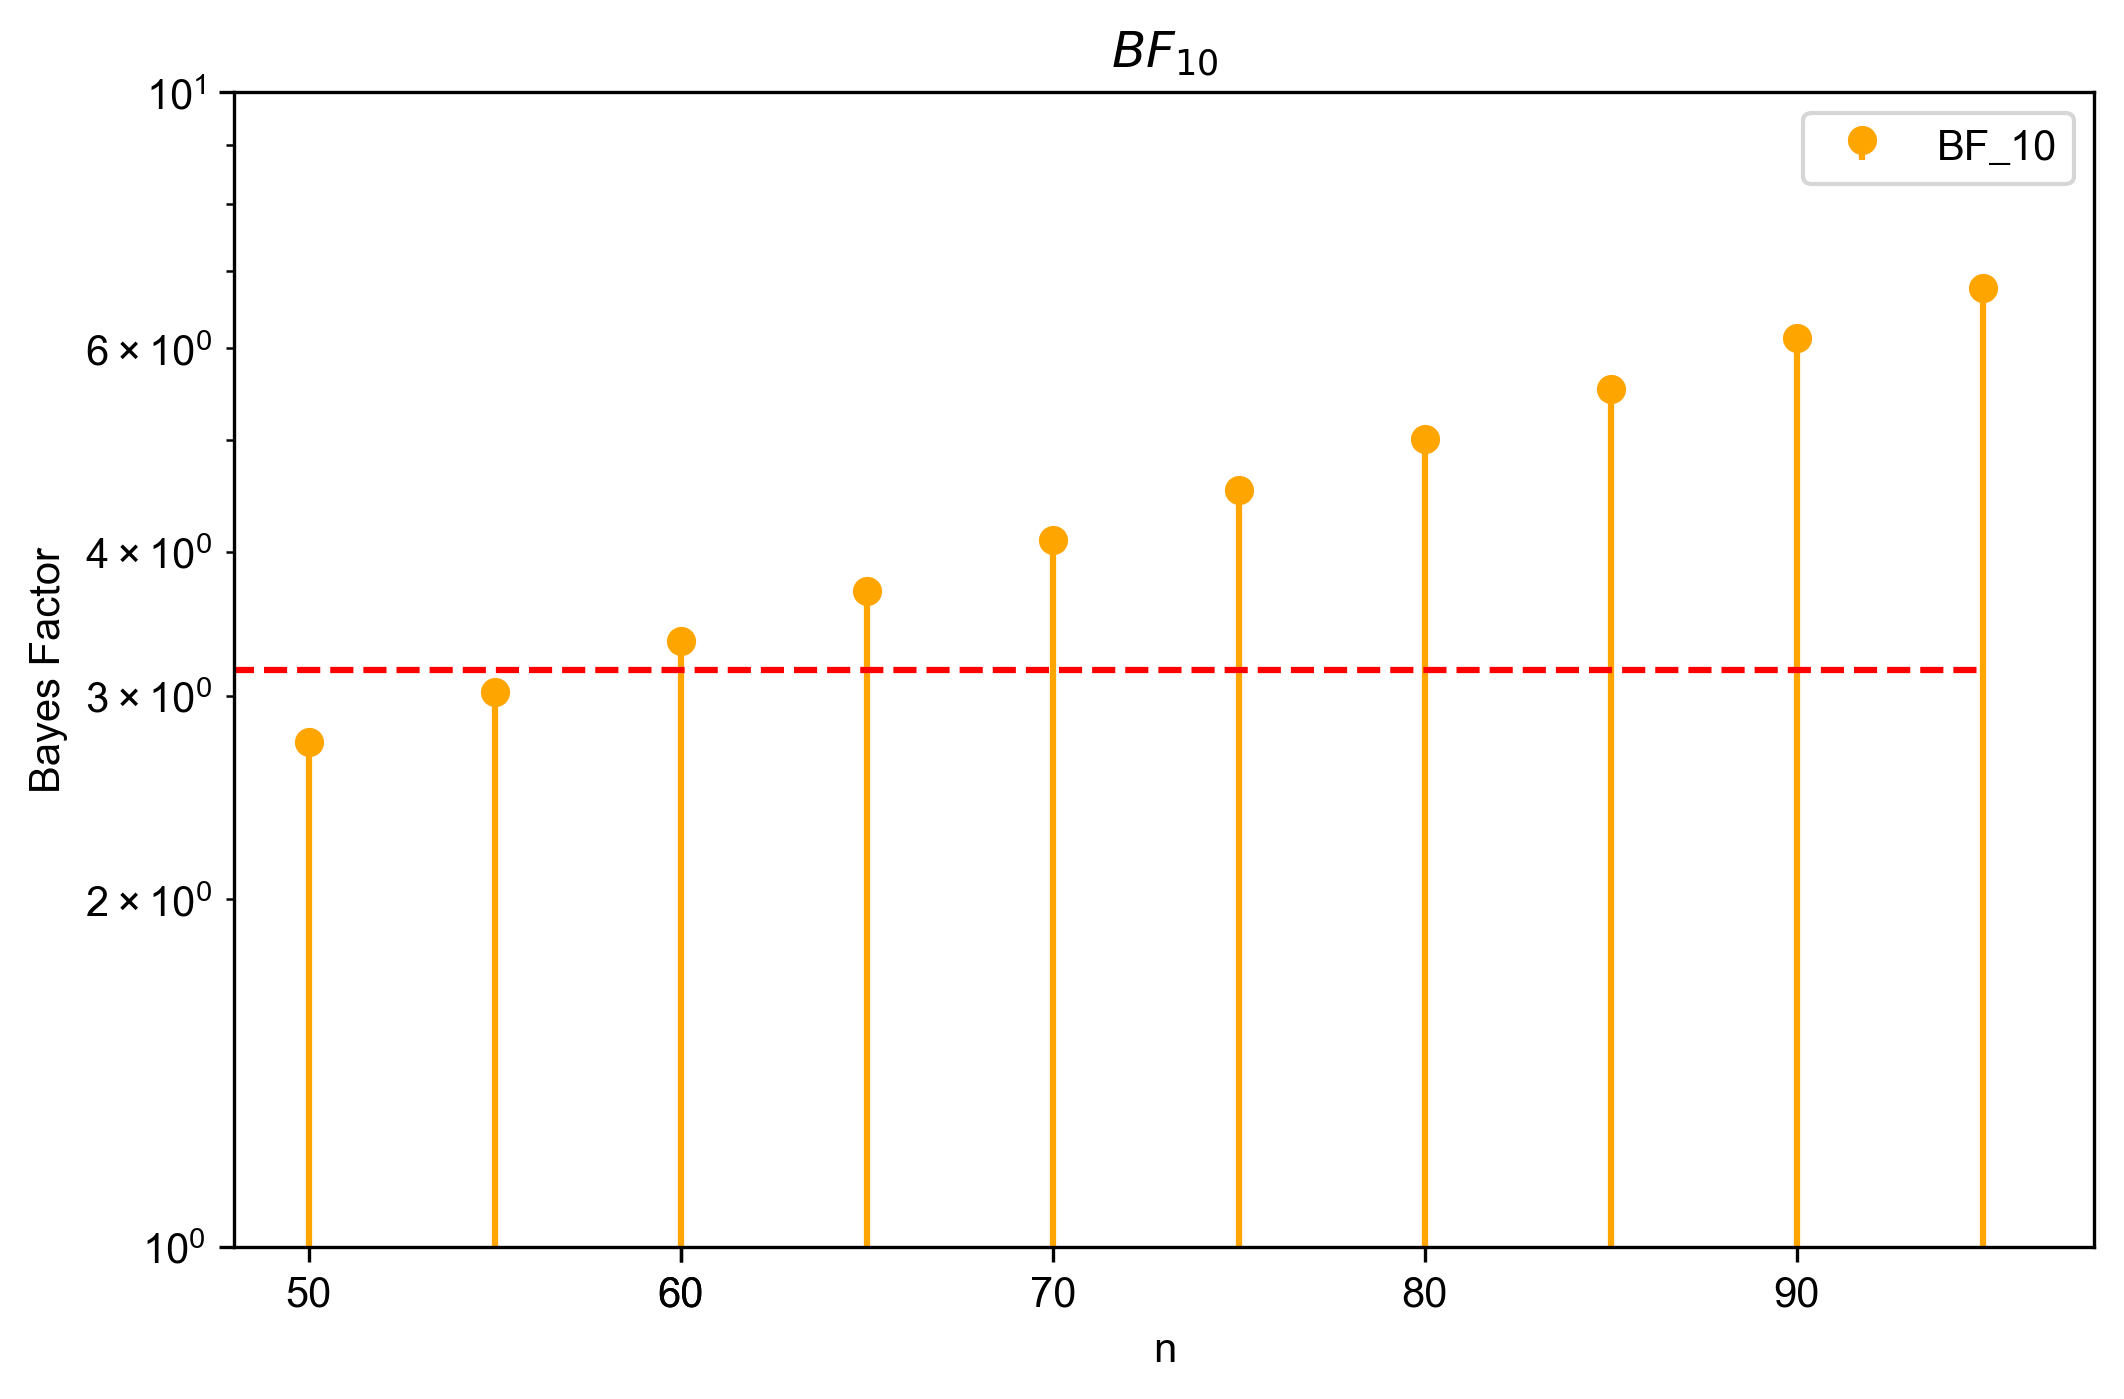
\includegraphics[width=0.7\linewidth]{figure/BF10.png} % 替换为实际图片路径
            \label{fig:BF10}
        }
        \caption{贝叶斯因子及\(BF_{10}\)随试验次数的变化曲线}
        \vspace{-2em}
    \end{figure}
    

\end{enumerate}

\appendix

\raggedright

\section{附录 A}

\noindent 计算\(\int_0^1 p^{0.4n} (1-p)^{0.6n} dp\)
\label{code1}
\begin{python}
    from sympy import *
    p = Symbol('x')
    n = Symbol('n')
    L_D_H2 = p**(0.4*n)*(1-p)**(0.6*n)
    P_D_H2 = integrate(L_D_H2, (p, 0, 1))
    P_D_H2._repr_latex_()
\end{python}

\section{附录 B}
\label{code2}
\noindent 计算\(BF_{12(n+5)}-BF_{12(n)}\)
\begin{python}
    from sympy import *
    from IPython.display import display, Math

    p = Symbol('p')
    n = Symbol('n', integer=True, positive=True, multiple_of=5)

    L_D_H2 = p**(0.4*n) * (1-p)**(0.6*n)
    P_D_H1 = 0.4**(0.4*n) * 0.6**(0.6*n)
    P_D_H2 = integrate(L_D_H2, (p, 0, 1))
    BF_12 = P_D_H1 / P_D_H2

    BF_12 = simplify(BF_12)
    BF_12 = BF_12.rewrite(gamma, factorial)

    Delta_BF_12 = BF_12.subs(n, n + 5) - BF_12.subs(n,n)

    display(Math(latex(Delta_BF_12)))
    print(latex(Delta_BF_12))
\end{python}

\section{附录 C}
\label{code3}
\noindent 用sympy判断正负性
\begin{python}
    numerator = (2*n + 4) * (2*n + 6) * (3*n + 12)  * (3*n + 18)
    denominator = (2*n + 5) * (2*n + 10) * (3*n + 5) * (3*n + 10) 
    f = numerator / denominator - 1
    from sympy.solvers.inequalities import reduce_inequalities

    positive = reduce_inequalities(f > 0, n)
    print("f(n) > 0 when:", positive)

    negative = reduce_inequalities(f < 0, n)
    print("f(n) < 0 when:", negative)
\end{python}

\section{附录 D}
\label{code4}
\noindent 计算贝叶斯因子随试验次数的变化曲线
\begin{python}
    from pylab import *
    from sympy import *
    import tqdm
    rcParams['font.sans-serif'] = ['Arial Unicode MS']
    BF_10 = np.array([])
    BF_20 = np.array([])
    BF_12 = np.array([])
    p = Symbol('x')
    N = np.arange(50, 400, 5)
    Flag = 0
    for n in tqdm.tqdm(N):
        L_D_H2 = np.power(p, int(0.4 * n)) * \
            np.power(1 - p, int(0.6 * n))
        P_D_H0 = np.power(0.5, n)
        P_D_H1 = np.power(0.4, 0.4 * n) * np.power(0.6, 0.6 * n)
        P_D_H2 = integrate(L_D_H2, (p, 0, 1))
        BF_10 = np.append(BF_10, P_D_H1 / P_D_H0)
        BF_20 = np.append(BF_20, P_D_H2 / P_D_H0)
        BF_12 = np.append(BF_12, P_D_H1 / P_D_H2)
        if Flag == 0:
            if P_D_H2 / P_D_H0 > np.power(10,0.5):
                print(n)
                Flag = 1
\end{python}


\end{document}
